% Options for packages loaded elsewhere
\PassOptionsToPackage{unicode}{hyperref}
\PassOptionsToPackage{hyphens}{url}
%
\documentclass[
]{article}
\usepackage{amsmath,amssymb}
\usepackage{lmodern}
\usepackage{iftex}
\ifPDFTeX
  \usepackage[T1]{fontenc}
  \usepackage[utf8]{inputenc}
  \usepackage{textcomp} % provide euro and other symbols
\else % if luatex or xetex
  \usepackage{unicode-math}
  \defaultfontfeatures{Scale=MatchLowercase}
  \defaultfontfeatures[\rmfamily]{Ligatures=TeX,Scale=1}
\fi
% Use upquote if available, for straight quotes in verbatim environments
\IfFileExists{upquote.sty}{\usepackage{upquote}}{}
\IfFileExists{microtype.sty}{% use microtype if available
  \usepackage[]{microtype}
  \UseMicrotypeSet[protrusion]{basicmath} % disable protrusion for tt fonts
}{}
\makeatletter
\@ifundefined{KOMAClassName}{% if non-KOMA class
  \IfFileExists{parskip.sty}{%
    \usepackage{parskip}
  }{% else
    \setlength{\parindent}{0pt}
    \setlength{\parskip}{6pt plus 2pt minus 1pt}}
}{% if KOMA class
  \KOMAoptions{parskip=half}}
\makeatother
\usepackage{xcolor}
\usepackage[margin=1in]{geometry}
\usepackage{graphicx}
\makeatletter
\def\maxwidth{\ifdim\Gin@nat@width>\linewidth\linewidth\else\Gin@nat@width\fi}
\def\maxheight{\ifdim\Gin@nat@height>\textheight\textheight\else\Gin@nat@height\fi}
\makeatother
% Scale images if necessary, so that they will not overflow the page
% margins by default, and it is still possible to overwrite the defaults
% using explicit options in \includegraphics[width, height, ...]{}
\setkeys{Gin}{width=\maxwidth,height=\maxheight,keepaspectratio}
% Set default figure placement to htbp
\makeatletter
\def\fps@figure{htbp}
\makeatother
\setlength{\emergencystretch}{3em} % prevent overfull lines
\providecommand{\tightlist}{%
  \setlength{\itemsep}{0pt}\setlength{\parskip}{0pt}}
\setcounter{secnumdepth}{-\maxdimen} % remove section numbering
\ifLuaTeX
  \usepackage{selnolig}  % disable illegal ligatures
\fi
\IfFileExists{bookmark.sty}{\usepackage{bookmark}}{\usepackage{hyperref}}
\IfFileExists{xurl.sty}{\usepackage{xurl}}{} % add URL line breaks if available
\urlstyle{same} % disable monospaced font for URLs
\hypersetup{
  pdftitle={``Supervised learning final project''},
  pdfauthor={Diego Cubides,Larry castro, Tomas Mendez},
  hidelinks,
  pdfcreator={LaTeX via pandoc}}

\title{``Supervised learning final project''}
\author{Diego Cubides,Larry castro, Tomas Mendez}
\date{2023-05-29}

\begin{document}
\maketitle

\hypertarget{abstract}{%
\subsection{Abstract}\label{abstract}}

The present report is based on the implementation of machine learning to
predict three types of environments using the KNN algorithm, decision
tree, random forest, and logistic regression. Data was collected from a
DHT11 sensor, which measures humidity and temperature, an RGB color
sensor TCS3200D TCS230, and a PT100 probe. RStudio was used to train the
models with a dataset, and then the prediction was implemented for new
data.

For data acquisition and communication, a robot controlled by an Arduino
was used, communicating via serial communication with the HC-05
Bluetooth module. This allowed the robot to move easily between
different environments and gather data characterizing each one.

Keywords: machine learning, predict, KNN algorithm, decision tree,
random forest, logistic regression, DHT11 sensor, humidity, temperature,
RGB color sensor TCS3200D TCS230, PT100 probe, RStudio, model training,
prediction of new data, data acquisition, serial communication, Arduino,
HC-05 Bluetooth module, robot, environments.

\hypertarget{resumen}{%
\subsection{Resumen}\label{resumen}}

El presente informe se centra en la aplicación del aprendizaje
automático para predecir tres tipos de ambientes utilizando los
algoritmos KNN, árbol de decisiones, bosque aleatorio y regresión
logística. Se recopilaron datos de un sensor DHT11 para medir la humedad
y la temperatura, un sensor de color RGB TCS3200D TCS230 y una sonda
PT100. Se utilizó RStudio para entrenar los modelos utilizando un
conjunto de datos y luego se implementó la predicción para nuevos datos.

Para la adquisición de datos y la comunicación, se utilizó un robot
controlado por un Arduino, que se comunicaba a través de la comunicación
serial con el módulo de Bluetooth HC-05. Esto permitió que el robot se
moviera fácilmente entre diferentes ambientes y recopilara los datos que
caracterizaban cada uno de ellos.

Palabras clave: aprendizaje de máquina, predecir, algoritmo Knn, árbol
de decisiones, bosque aleatorio, regresión logística, sensor DHT11,
humedad, temperatura, sensor de color RGB TCS3200D TCS230, sonda PT100,
RStudio, entrenamiento de modelos, prediccion de nuevos datos,
adquisición de datos, comunicación serial, Arduino, módulo de Bluetooth
HC-05, robot, ambientes.

\hypertarget{introduccion}{%
\subsection{Introduccion}\label{introduccion}}

El aprendizaje de máquina y sus modelos, como KNN, árbol de decisiones,
bosque aleatorio y regresión logística, son vitales en la actualidad.
Estos modelos permiten resolver problemas complejos y tomar decisiones
precisas. KNN clasifica ejemplos según su proximidad, mientras que el
árbol de decisiones utiliza reglas jerárquicas. El bosque aleatorio
combina múltiples árboles para mayor precisión, y la regresión logística
predice probabilidades binarias. Estos modelos analizan grandes
volúmenes de datos, revelando patrones ocultos y haciendo predicciones
en diversos campos, desde medicina hasta finanzas. Su importancia radica
en mejorar la toma de decisiones y generar conocimientos valiosos.

\hypertarget{materiales}{%
\subsection{Materiales}\label{materiales}}

\begin{itemize}
\tightlist
\item
  Sensor de color RGB TCS3200D TCS230
\item
  Sensor DHT11
\item
  Sonda PT100
\item
  Modulo puente h l298n
\item
  Carro a control remoto
\item
  Bluetooth hc-05
\item
  Arduino UNO
\item
  Dispositivo Android
\end{itemize}

\hypertarget{software}{%
\subsection{Software}\label{software}}

\begin{itemize}
\item
  RStudio
\item
  Arduino
\item
  App inventor
\item
  Excel
\item
  PLX-DAQ
\end{itemize}

\hypertarget{procedimiento}{%
\subsection{Procedimiento}\label{procedimiento}}

\hypertarget{adquisision-de-datos}{%
\subsubsection{adquisision de datos}\label{adquisision-de-datos}}

Se desarrolló un sistema de control remoto para un carro mediante la
tecnología Bluetooth, el cual posee la capacidad de moverse a diferentes
velocidades y en múltiples direcciones. Para lograr esto, se creó una
aplicación utilizando App Inventor, que permite el control preciso del
movimiento del carro y la transmisión de datos en tiempo real. La app
facilita la interacción con el carro y la recepción de los datos
capturados en cada instante.

\begin{figure}
\centering
\includegraphics[width=2.03125in,height=0.9375in]{app.png}
\caption{App}
\end{figure}

\begin{figure}
\centering
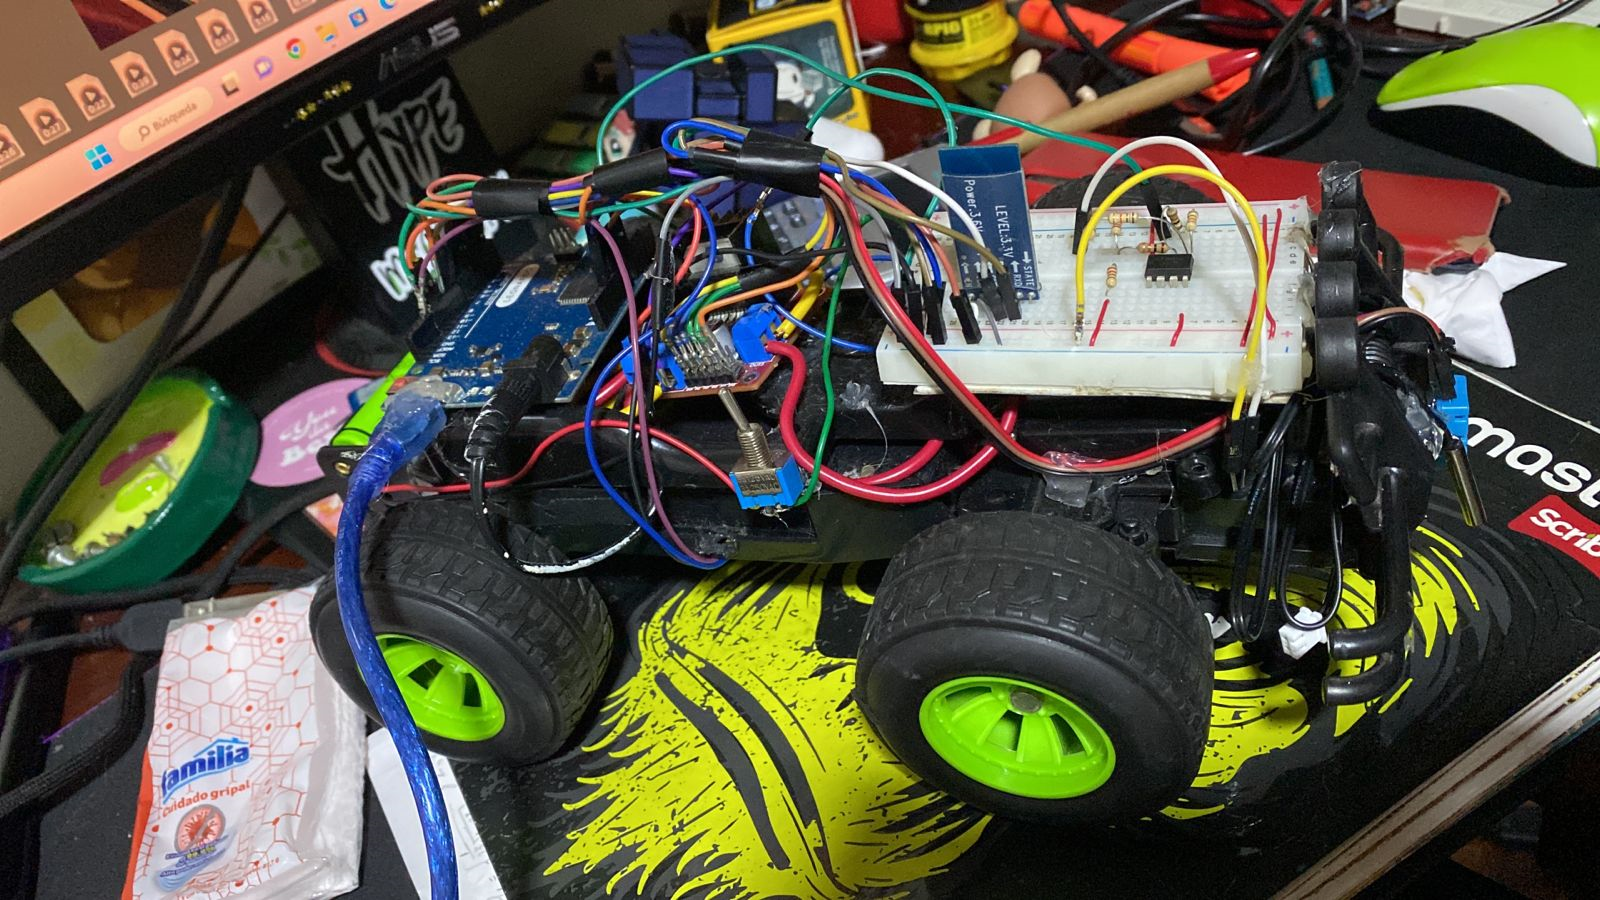
\includegraphics[width=2.04167in,height=\textheight]{robot.png}
\caption{Robot}
\end{figure}

Para la adquisición de datos en tiempo real, se empleó el programa
PLX-DAQ, el cual facilita la comunicación entre los datos provenientes
del Arduino y Microsoft Excel. Esta integración permitió abrir los datos
en RStudio como un archivo CSV, lo que posibilitó su posterior análisis
y procesamiento.

\begin{figure}
\centering
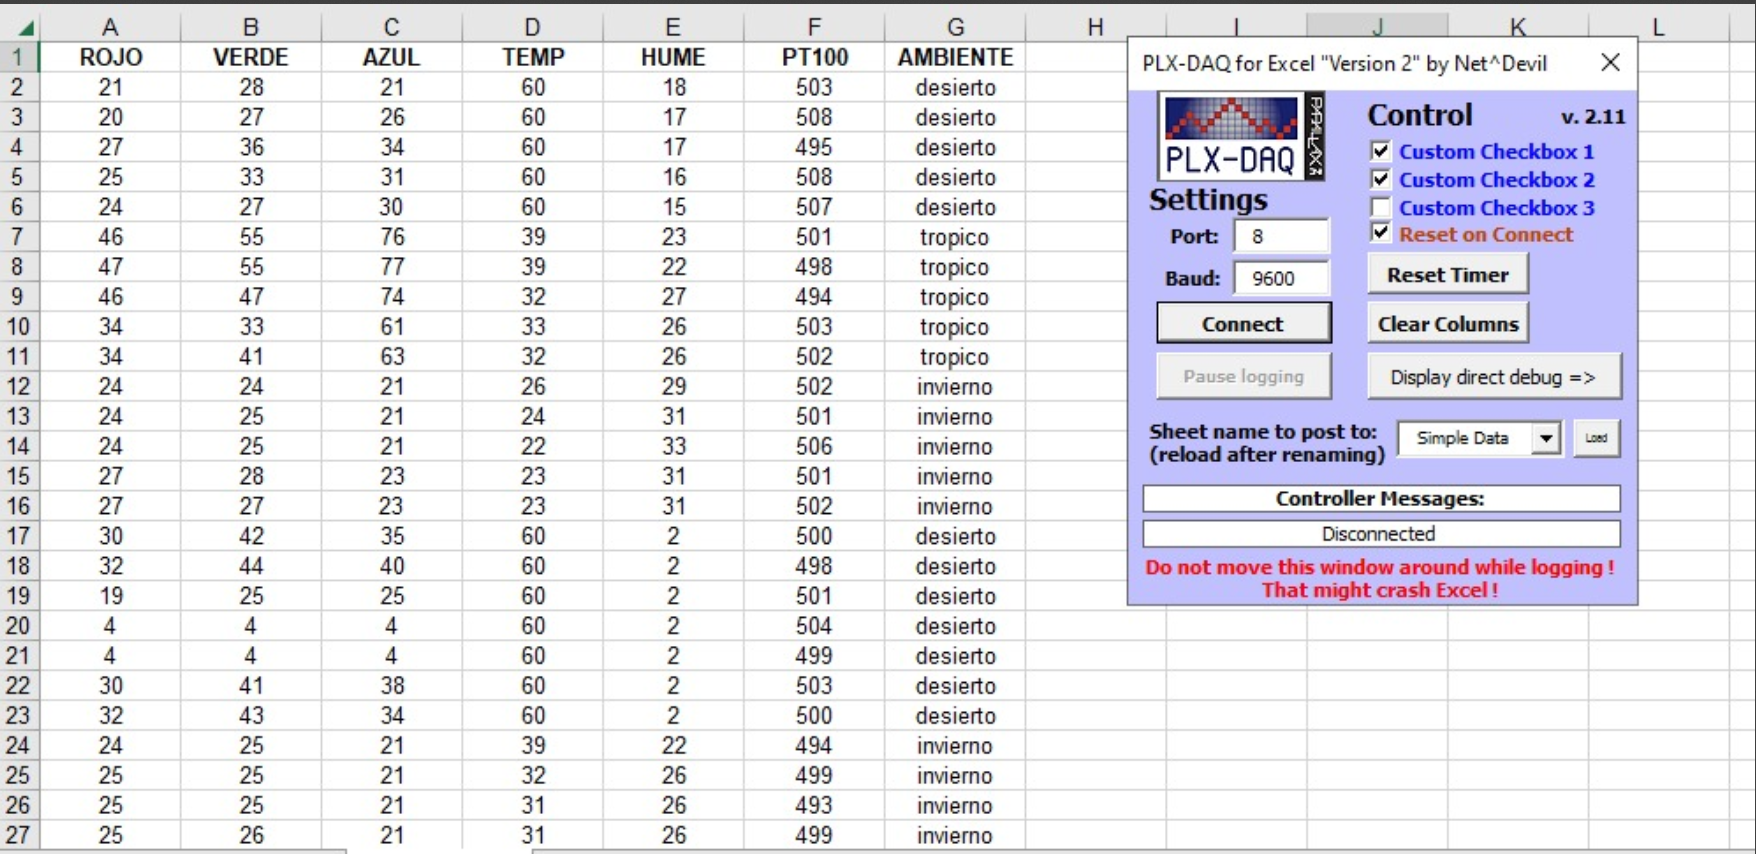
\includegraphics[width=2.03125in,height=0.9375in]{PLX.png}
\caption{PLX-DQ}
\end{figure}

\hypertarget{entrenamiento-e-implementacion-de-los-modelos}{%
\subsubsection{Entrenamiento e implementacion de los
modelos}\label{entrenamiento-e-implementacion-de-los-modelos}}

\end{document}
